\documentclass[11pt]{article}

\usepackage{amsmath,amssymb,amsthm}
\usepackage{booktabs}
\usepackage{geometry}
\usepackage{hyperref}
\usepackage{xurl}
\usepackage{tikz}

\geometry{margin=1in}

\newtheorem{theorem}{Theorem}
\newtheorem{lemma}[theorem]{Lemma}
\newtheorem{proposition}[theorem]{Proposition}
\newtheorem{corollary}[theorem]{Corollary}
\newtheorem{definition}[theorem]{Definition}
\newtheorem{remark}[theorem]{Remark}

\title{Exact Pebbling Numbers of Double-Tailed Tadpole Graphs}
\author{Runze Yu}
\date{}

\begin{document}

\maketitle

\begin{abstract}
A path on $d+1$ vertices has pebbling number $2^d$.
Attach a unit-weight branch at the triangle apex of a double-tailed tadpole, and the
number rises by exactly one pebble.
We prove $\pi(T(3,s_1,s_2))=2^{s_1+s_2+1}+1$ for all $s_1,s_2\ge1$, where
$T(3,s_1,s_2)$ is a triangle with pendant paths of lengths $s_1,s_2$ to the
leaves $u_L$ and~$u_R$.
The lower bound is witnessed by placing $2^d-1$ pebbles on the farther leaf and one
on the apex; the upper bound uses a path-spine weight function with that same apex
branch.
Small instances agree with the formula under exhaustive search.
\end{abstract}

% Introduction

\section{Introduction}\label{sec:intro}

In \emph{graph pebbling}, a move along edge $\{u,v\}$ removes two pebbles from~$u$ and
places one on~$v$.
The \emph{pebbling number} $\pi(G)$ is the smallest~$S$ for which every $S$-pebble
configuration can reach every target~\cite{Chung1989,HurlbertKenter2021}.
One always has $\pi(G)\ge |V(G)|$ and $\pi(G)\ge 2^{\operatorname{diam}(G)}$; on a path
$P_{d+1}$ the value is exactly $2^d$~\cite{Hurlbert1999,AlconHurlbert2022}.
Upper bounds often come from \emph{weight functions}~\cite{Hurlbert2017,YYZ2024}: if
$w(1_G)=2^d$, the minimum off-target weight is~$1$, and $w$ is valid, then
$\pi(G)\le 2^d+1$.

The graph $T(3,s_1,s_2)$ is a triangle on $\{a,b,c\}$ with paths of lengths $s_1$ and
$s_2$ from~$a$ and~$b$ to leaves $u_L$ and~$u_R$; the apex~$c$ carries no tail
(Definition~\ref{sec:tadpole-def}, Figure~\ref{fig:tadpole-schematic}).
Its diameter is $d=s_1+s_2+1$.
Closed formulas for classical tadpoles under standard moves are rare; much of the
literature under that name treats \emph{monophonic} pebbling~\cite{Iammal2026}, where
moves are confined to longest chordless paths.

Our main result (Theorem~\ref{thm:exact}) is
\[
\pi\bigl(T(3,s_1,s_2)\bigr)=2^d+1
\quad\text{for all } s_1,s_2\ge1,
\]
one pebble above the path bound $2^d$.
We do not know of an earlier exact formula for a two-parameter family of
double-tailed graphs with a triangle core under standard moves.

Section~\ref{sec:preliminaries} fixes notation and the critical configuration~$D^*$.
Section~\ref{sec:lemmas} shows that only the two leaves matter as targets.
The proof of the closed formula occupies Sections~\ref{sec:aux-bounds}--\ref{sec:upper-bound};
Section~\ref{sec:computational} and Appendix~\ref{sec:appendix-computational} record
small-instance searches that were run while the argument was being tested.

\medskip
\noindent\textbf{Keywords.} graph pebbling; pebbling number; tadpole graph; weight function.

\medskip
\noindent\textbf{MSC 2020.} 05C57 (Primary); 05C35 (Secondary).

% Preliminaries: definitions and notation

\section{Preliminaries}\label{sec:preliminaries}

\subsection{Graph pebbling}

Let $G=(V,E)$ be a connected graph.
A \emph{pebble configuration} is a function $p\colon V\to\mathbb{Z}_{\ge 0}$.
A \emph{pebbling move} on an edge $\{u,v\}$ is allowed when $p(u)\ge 2$ and replaces
$p$ by $p'$ with $p'(u)=p(u)-2$, $p'(v)=p(v)+1$, and $p'(w)=p(w)$ for $w\notin\{u,v\}$.
We say that a configuration $p$ can \emph{pebble} (or \emph{reach}) a target vertex $t$
if some finite sequence of pebbling moves produces a configuration with at least one pebble on~$t$.

For a fixed target $t$, the \emph{$t$-pebbling number} is
\[
\pi(G,t)=\min\{S\in\mathbb{Z}_{>0} : \text{every configuration with exactly $S$ pebbles can pebble $t$}\}.
\]
The \emph{pebbling number} of $G$ is
\[
\pi(G)=\max_{t\in V}\pi(G,t).
\]

\begin{lemma}[Monotonicity {\cite[Prop.~2]{Bunde2008}}]\label{lem:mono}
Fix a target~$t$. If $k\ge \pi(G,t)$, then every configuration with exactly $k$
pebbles can pebble~$t$.
\end{lemma}

\begin{proof}
See~\cite{Bunde2008,Hurlbert1999}.
\end{proof}

\subsection{Double-tailed tadpole graphs}\label{sec:tadpole-def}

\begin{definition}[Double-tailed tadpole graph $T(3,s_1,s_2)$]
Fix integers $s_1,s_2\ge 1$.
The graph $T(3,s_1,s_2)$ consists of:
\begin{itemize}
  \item a triangle on vertices $\{a,b,c\}$;
  \item a path of length $s_1$ joining $a$ to a leaf $u_L$;
  \item a path of length $s_2$ joining $b$ to a leaf $u_R$;
  \item no edges from $c$ to either tail.
\end{itemize}
The graph has $n=3+s_1+s_2$ vertices and diameter
\[
d=s_1+s_2+1=\operatorname{diam}(T(3,s_1,s_2)).
\]
\end{definition}

\begin{figure}[ht]
\centering
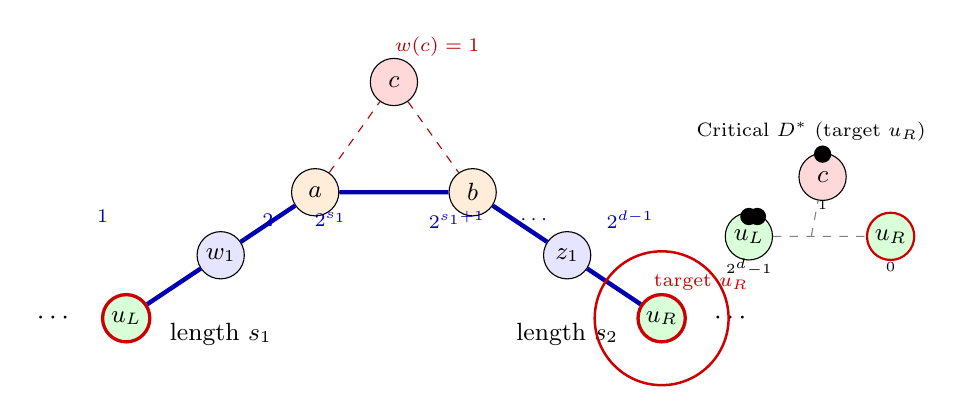
\begin{tikzpicture}[
  vtx/.style={circle, draw, minimum size=6mm, inner sep=0pt, font=\small},
  tail/.style={vtx, fill=blue!10},
  tri/.style={vtx, fill=orange!15},
  apex/.style={vtx, fill=red!15},
  leaf/.style={vtx, fill=green!15},
  target/.style={leaf, draw=red!80!black, line width=1.2pt},
  spine/.style={line width=1.6pt, draw=blue!70!black},
  branch/.style={dashed, draw=red!70!black},
  peb/.style={circle, fill=black, inner sep=0pt, minimum size=2.2mm}
]
  \node[tri] (a) at (0,0) {$a$};
  \node[tri] (b) at (2,0) {$b$};
  \node[apex] (c) at (1,1.4) {$c$};
  \draw (a)--(b);
  \draw[branch] (a)--(c)--(b);
  \node[tail] (w1) at (-1.2,-0.8) {$w_1$};
  \node[target] (uL) at (-2.4,-1.6) {$u_L$};
  \draw[spine] (uL)--(w1)--(a)--(b);
  \node at (-3.3,-1.6) {$\cdots$};
  \node at (-1.2,-1.8) {\small length $s_1$};
  \node[tail] (z1) at (3.2,-0.8) {$z_1$};
  \node[target] (uR) at (4.4,-1.6) {$u_R$};
  \draw[spine] (b)--(z1)--(uR);
  \node at (5.3,-1.6) {$\cdots$};
  \node at (3.2,-1.8) {\small length $s_2$};
  \node[font=\scriptsize, blue!70!black] at (-2.7,-0.3) {$1$};
  \node[font=\scriptsize, blue!70!black] at (-0.6,-0.35) {$2$};
  \node[font=\scriptsize, blue!70!black] at (0.2,-0.35) {$2^{s_1}$};
  \node[font=\scriptsize, blue!70!black] at (1.8,-0.35) {$2^{s_1+1}$};
  \node[font=\scriptsize, blue!70!black] at (2.8,-0.35) {$\cdots$};
  \node[font=\scriptsize, blue!70!black] at (4.0,-0.35) {$2^{d-1}$};
  \node[font=\scriptsize, red!70!black] at (1.55,1.85) {$w(c)=1$};
  \node[font=\scriptsize, red!80!black] at (4.9,-1.15) {target $u_R$};
  \draw[red!80!black, line width=0.9pt] (4.4,-1.6) circle (8.5mm);

  \begin{scope}[shift={(6.3,-0.2)}, scale=0.72]
    \node[font=\scriptsize] at (0,1.35) {Critical $D^*$ (target $u_R$)};
    \node[vtx, fill=green!15] (duL) at (-1.1,-0.5) {$u_L$};
    \node[vtx, fill=red!15] (dc) at (0.2,0.55) {$c$};
    \node[vtx, fill=green!15, draw=red!80!black, line width=0.8pt] (duR) at (1.4,-0.5) {$u_R$};
    \draw[dashed, gray] (duL)--(0,-0.5)--(duR);
    \draw[dashed, gray] (0,-0.5)--(dc);
    \node[font=\tiny] at (-1.1,-1.05) {$2^d{-}1$};
    \node[font=\tiny] at (0.2,0.05) {$1$};
    \node[font=\tiny] at (1.4,-1.05) {$0$};
    \node[peb] at (-1.1,-0.15) {};
    \node[peb] at (-0.95,-0.15) {};
    \node[peb] at (0.2,0.95) {};
  \end{scope}
\end{tikzpicture}
\caption{$T(3,s_1,s_2)$ and the objects used later.
The bold spine is the Hamiltonian path $u_L\to\cdots\to u_R$ of
Section~\ref{sec:path-spine-wf}; dashed edges mark the branch at~$c$.
Blue labels are path-spine weights toward target~$u_R$ (red circle).
The inset shows the critical configuration~$D^*$ (Definition~\ref{def:critical}).}
\label{fig:tadpole-schematic}
\end{figure}

\subsection{Critical configuration}\label{sec:critical-def}

\begin{definition}[Critical configuration $D^*$]\label{def:critical}
Fix target $u_R$ and let $d=s_1+s_2+1$.
Define the configuration $D^*$ by
\[
D^*(u_L)=2^d-1,\qquad D^*(c)=1,\qquad D^*(v)=0 \text{ for all other vertices } v.
\]
Then $|D^*| = 2^d$.
\end{definition}

At $S=2^d$, every instance in Table~\ref{tab:critical} fails in a configuration
matching~$D^*$ up to automorphism.
That $D^*$ cannot pebble~$u_R$ is proved in Section~\ref{sec:lower-bound}; the value
$\pi(G)=2^d+1$ is Theorem~\ref{thm:exact}.


\section{Structural lemmas}\label{sec:lemmas}
% Leaf Target Sufficiency Lemma

\subsection{Leaf target sufficiency}\label{sec:leaf-lemma}

The solver in Section~\ref{sec:computational} tests only the leaf targets $u_L$ and~$u_R$.

\begin{lemma}[Leaf target sufficiency]\label{lem:leaf}
Let $G=T(3,s_1,s_2)$ with leaves $u_L$ and $u_R$. Then
\[
\pi(G)=\max\bigl\{\pi(G,u_L),\,\pi(G,u_R)\bigr\}.
\]
Equivalently, if every configuration with $S$ pebbles can pebble both leaves,
then every such configuration can pebble every vertex of~$G$.
\end{lemma}

\begin{lemma}[Tail propagation]\label{lem:tail-prop}
Let $P=(w_0,w_1,\ldots,w_k)$ be a path in $G$ with $w_k$ a leaf of~$G$.
For every $i\in\{0,1,\ldots,k\}$,
\[
\pi(G,w_i)\le \pi(G,w_k).
\]
In particular, with $P_L=(a,\ldots,u_L)$ and $P_R=(b,\ldots,u_R)$ one has
$\pi(G,v)\le \pi(G,u_L)$ for every vertex $v$ on the left tail and
$\pi(G,v)\le \pi(G,u_R)$ for every vertex $v$ on the right tail.
\end{lemma}

\begin{lemma}[First double on a path]\label{lem:first-double}
Let $P=(w_0,w_1,\ldots,w_k)$ be a path and let $D$ be a configuration that
pebbles~$w_i$ for some $i\in\{0,1,\ldots,k\}$.
If some reachable state satisfies $p(w_i)\ge 2$, then $D$ pebbles~$w_i$.
Otherwise $p(w_i)\le 1$ in every reachable state, and the first move that
places a pebble on~$w_i$ is either $w_{i-1}\to w_i$ (when $i\ge 1$) or
$w_{i+1}\to w_i$ (when $i\le k-1$); in either case the prefix ending
immediately before that move already places at least two pebbles on the source
vertex, so $D$ pebbles that source as well.
\end{lemma}

\begin{proof}
If a reachable state has $p(w_i)\ge 2$, then either $w_i\to w_{i-1}$ or
$w_i\to w_{i+1}$ is legal toward pebbling a neighbor, and the claim is
immediate from the definition of ``$D$ pebbles~$w_i$''.

Assume $p(w_i)\le 1$ in every reachable state.
Let $m$ be the first move in a pebbling sequence for~$w_i$ that places a pebble
on~$w_i$.
Because $p(w_i)=0$ before~$m$, the move $m$ is either $w_{i-1}\to w_i$ or
$w_{i+1}\to w_i$.
Each requires at least two pebbles on its source immediately beforehand, and
the prefix ending before~$m$ pebbles that source.
\end{proof}

\begin{lemma}[Left junction supply for the apex]\label{lem:left-junction}
Let $G=T(3,s_1,s_2)$ and let $w_1$ denote the neighbor of~$a$ on the left
tail ($w_1=u_L$ when $s_1=1$).
Fix a configuration~$p$ that can pebble~$a$.
If every reachable configuration has $p(c)=0$ and $p(b)\le 1$, then some
reachable configuration~$p'$ satisfies $p'(a)\ge 2$.
\end{lemma}

\begin{proof}
If some reachable state already has $p(a)\ge 2$, we are done.
Assume $p(a)\le 1$ in every reachable state.
Because $p$ pebbles~$a$, some sequence ends with a pebble on~$a$.

The first move~$m$ that places a pebble on~$a$ cannot be $c\to a$ or $b\to a$,
because $p(c)=0$ and $p(b)\le 1$ in every reachable state.
Hence $m=w_1\to a$, and the prefix ending immediately before~$m$ already has
$p(w_1)\ge 2$ by Lemma~\ref{lem:first-double}.

If $p(a)=0$ before~$m$, then after~$m$ we have $p(a)=1$.
Because $p(a)\le 1$ always, a second move must place another pebble on~$a$;
it is again $w_1\to a$, and immediately beforehand $p(w_1)\ge 2$.
Performing this second move yields a reachable state with $p(a)\ge 2$.
\end{proof}

\begin{proof}[Proof of Lemma~\ref{lem:tail-prop}]
Fix $S=\pi(G,w_k)$ and let $D$ be any configuration with $|D|=S$.
We prove by downward induction on $i$ that $D$ pebbles~$w_i$.

The base $i=k$ is immediate.
For $i<k$, assume $D$ pebbles~$w_{i+1}$.
If $D$ already pebbles~$w_i$, we are done.
Otherwise $p(w_i)=0$.

\smallskip\noindent
\textbf{Cases 1--2.}
If $p(w_{i+1})=0$, the first move placing a pebble on~$w_{i+1}$ is $w_i\to w_{i+1}$,
and its prefix pebbles~$w_i$.
If $p(w_{i+1})\ge 2$, then $w_{i+1}\to w_i$ pebbles~$w_i$.

\smallskip\noindent
\textbf{Case 3: $p(w_{i+1})=1$ and $p(w_i)=0$.}
Suppose $D$ does not pebble~$w_i$.

If some sequence raises $p(w_{i+1})$ to~$2$, let $m$ be the first such move.
Then $m$ is $w_i\to w_{i+1}$ or $w_{i+2}\to w_{i+1}$ (when $i+2\le k$).
In the first case the prefix before~$m$ already places two pebbles on~$w_i$.
In the second case, apply the same first-double chase on the suffix
$(w_{i+1},\ldots,w_k)$: when $i=k-1$ the only possible first accumulation is
$w_{k-1}\to w_k$, whose prefix pebbles $w_{k-1}=w_i$; for $i<k-1$, iterate until
a prefix pebbles~$w_i$.
Both contradict the assumption that $D$ does not pebble~$w_i$.

Hence $p(w_{i+1})\le 1$ in every reachable state, so neither
$w_{i+1}\to w_i$ nor $w_{i+1}\to w_{i+2}$ is ever legal.

If $i=k-1$, then $w_{i+1}=w_k$ is the leaf.
The lone pebble on~$w_k$ cannot be inert, for otherwise $|D|-1$ pebbles would
suffice to pebble~$w_k$, contradicting $S=\pi(G,w_k)$.
Some sequence therefore executes $w_{k-1}\to w_k$, and the prefix before that move
places at least two pebbles on~$w_{k-1}=w_i$ (Lemma~\ref{lem:first-double}).

If $i<k-1$, no sequence can use $w_{k-1}\to w_k$, for that would force
$p(w_{i+1})\ge 2^{\,k-i-1}$ by Lemma~\ref{lem:path-lb} on the subpath
$(w_{i+1},\ldots,w_k)$, contradicting the paragraph above.
Because $D$ pebbles~$w_{k-1}$, the first move placing a pebble on~$w_{k-1}$ is either
$w_{k-2}\to w_{k-1}$ or $w_k\to w_{k-1}$; in either case the prefix before that move
pebbles a neighbor closer to~$w_i$, and repeating the first-double chase along
$(w_i,\ldots,w_{k-1})$ eventually yields a prefix that pebbles~$w_i$ or a move
$w_i\to w_{i+1}$ whose prefix pebbles~$w_i$.

In every subcase, $D$ pebbles~$w_i$.
Thus $\pi(G,w_i)\le S=\pi(G,w_k)$ for every $i\in\{0,\ldots,k\}$.
\end{proof}

\begin{lemma}[Triangle access to the apex]\label{lem:triangle-apex}
Let $G=T(3,s_1,s_2)$ and let $D$ be a configuration with $|D|=\pi(G,u_R)$
that can pebble~$u_R$.
If $p(c)=0$ in every reachable state and $p(b)\le 1$ in every reachable state,
then $D$ can pebble~$c$.
\end{lemma}

\begin{proof}
If some reachable state has $p(b)\ge 2$, then $b\to c$ places a pebble on~$c$.
Assume $p(b)\le 1$ in every reachable state, so $b\to c$ is never legal and any
pebbling of~$c$ must use $a\to c$, which requires a reachable state with
$p(a)\ge 2$.
Because $\pi(G,a)\le \pi(G,u_R)=|D|$, configuration~$D$ can pebble~$a$.
Since $p(c)=0$ and $p(b)\le 1$ in every reachable state,
Lemma~\ref{lem:left-junction} gives a reachable state~$\sigma$ with
$\sigma(a)\ge 2$, and then $a\to c$ pebbles~$c$.

In every subcase, $D$ can pebble~$c$.
\end{proof}

\begin{lemma}[Apex bound]\label{lem:apex-bound}
The triangle apex satisfies
\[
\pi(G,c)\le \max\bigl\{\pi(G,u_L),\,\pi(G,u_R)\bigr\}.
\]
\end{lemma}

\begin{proof}
By symmetry, assume $\pi(G,u_R)\ge \pi(G,u_L)$.
Let $D$ be any configuration with $|D|=\pi(G,u_R)$ pebbles.
Then $D$ can pebble~$u_R$.

If $D$ already places a pebble on~$c$, then $\pi(G,c)\le \pi(G,u_R)$.

Otherwise $p(c)=0$.
We show that $D$ can pebble~$c$.

\smallskip\noindent
\textbf{Case 1: $p(u_R)=0$ in~$D$.}
Choose a pebbling sequence from~$D$ that places a pebble on~$u_R$.
Since $p(u_R)=0$, Lemma~\ref{lem:path-lb} applied to the right tail yields a reachable
configuration~$\sigma$ with $\sigma(b)\ge 2^{s_2}$.
If $\sigma(c)\ge 1$, then $D$ pebbles~$c$.
Otherwise the move $b\to c$ is legal in~$\sigma$ and places a pebble on~$c$.

\smallskip\noindent
\textbf{Case 2: $p(u_R)\ge 1$ in~$D$.}
Then $D$ already pebbles~$u_R$ by the empty sequence.
If some reachable state~$\sigma$ satisfies $\sigma(b)\ge 2$ or $\sigma(a)\ge 2$,
then a single move $b\to c$ or $a\to c$ pebbles~$c$.
Otherwise $p(a)\le 1$, $p(b)\le 1$, and $p(c)=0$ in every reachable state.
These are exactly the hypotheses of Lemma~\ref{lem:triangle-apex}, so $D$ can
pebble~$c$ by that lemma.

\smallskip\noindent
In both cases, every configuration with $\pi(G,u_R)$ pebbles can pebble~$c$, so
$\pi(G,c)\le \pi(G,u_R)=\max\{\pi(G,u_L),\pi(G,u_R)\}$.
\end{proof}

\begin{proof}[Proof of Lemma~\ref{lem:leaf}]
By Lemma~\ref{lem:tail-prop}, every vertex on the left tail, including~$a$, satisfies
$\pi(G,v)\le \pi(G,u_L)$; every vertex on the right tail, including~$b$, satisfies
$\pi(G,v)\le \pi(G,u_R)$.
By Lemma~\ref{lem:apex-bound},
$\pi(G,c)\le \max\{\pi(G,u_L),\pi(G,u_R)\}$.
Therefore every vertex $t$ satisfies
\[
\pi(G,t)\le \max\bigl\{\pi(G,u_L),\,\pi(G,u_R)\bigr\}.
\]
The reverse inequality is immediate because $u_L$ and $u_R$ are vertices of~$G$.
\end{proof}

\begin{corollary}[Solver pruning]\label{cor:pruning}
The pebbling number of $T(3,s_1,s_2)$ equals the minimum $S$ such that every
configuration with $S$ pebbles can pebble both leaves.
\end{corollary}

\begin{table}[ht]
\centering
\caption{Per-target pebbling numbers from exhaustive search
(\texttt{verify\_leaf\_lemma.py}).}
\label{tab:leaf-verify}
\begin{tabular}{lrrrrrrr}
\hline
Graph & $d$ & $\pi(G,c)$ & $\pi(G,a)$ & $\pi(G,b)$ & $\pi(G,u_L)$ & $\pi(G,u_R)$ & $\pi(G)$ \\
\hline
$T(3,1,1)$ & 3 & 7  & 6  & 6  & 9  & 9  & 9  \\
$T(3,1,2)$ & 4 & 11 & 10 & 8  & 17 & 17 & 17 \\
$T(3,2,2)$ & 5 & 15 & 12 & 12 & 33 & 33 & 33 \\
$T(3,1,3)$ & 5 & 19 & 18 & 12 & 33 & 33 & 33 \\
\hline
\end{tabular}
\end{table}

Each row agrees with Lemmas~\ref{lem:leaf} and~\ref{lem:apex-bound}.
On $T(3,1,1)$, $\pi(G,c)=7$ lies strictly below both leaf values.
Output: \path{data/leaf_lemma_verification.json}.


% Computational results

\section{Computational Results}\label{sec:computational}

Nothing in this section is used in the proofs of Section~\ref{sec:proofs}.
The searches below were run while the closed formula was being checked on small
instances; scripts and logs are described in Section~\ref{sec:data-availability}.

\subsection{Methodology}

For each $G=T(3,s_1,s_2)$ we built an exhaustive solver (\texttt{pebbling\_solver.py})
with two cuts: leaf-target pruning (Lemma~\ref{lem:leaf}) and quotienting by
$\operatorname{Aut}(G)$.
Starting from a diameter-based lower bound on~$S$, the program lists $S$-pebble
multisets, tests reachability by breadth-first search on the pebbling state graph,
and returns the least~$S$ for which every leaf target is reachable from every
configuration.

\subsection{Verified instances}

Table~\ref{tab:results} lists completed runs.

\begin{table}[ht]
\centering
\caption{Exact pebbling numbers and worst failing configurations (target~$u_R$).
Vertex order: $0=a$, $1=b$, $2=c$, left tail, then right tail.}
\label{tab:results}
\begin{tabular}{lrrrrl}
\hline
Graph & $d$ & $|V|$ & $\pi(G)$ & $2^d{+}1$ & Worst config at $S=2^d$ \\
\hline
$T(3,1,1)$ & 3 & 5 & 9  & 9  & $(a,b,c,u_L,u_R)=(0,0,1,7,0)$ \\
$T(3,1,2)$ & 4 & 6 & 17 & 17 & $(a,b,c,u_L,z_1,u_R)=(0,0,1,15,0,0)$ \\
$T(3,2,2)$ & 5 & 7 & 33 & 33 & $(a,b,c,w_1,u_L,z_1,u_R)=(0,0,1,0,31,0,0)$ \\
$T(3,1,3)$ & 5 & 7 & 33 & 33 & $(a,b,c,u_L,z_1,z_2,u_R)=(0,0,1,31,0,0,0)$ \\
\hline
\end{tabular}
\end{table}

Both $T(3,2,2)$ and $T(3,1,3)$ have $d=5$ but different shape; in each case
$\pi(G)=33=2^5+1$.
Every worst configuration at $S=2^d$ matches~$D^*$ up to automorphism.

\subsection{Critical configurations at \texorpdfstring{$S=2^d$}{S=2 to the d}}

Table~\ref{tab:critical} gives one failing configuration at $S=2^d$ per instance
(target~$u_R$).

\begin{table}[ht]
\centering
\caption{Configurations witnessing $\pi(G)>2^d$.}
\label{tab:critical}
\begin{tabular}{lrrll}
\hline
Graph & $d$ & $S$ fails & Target $u_R$ & Config tuple \\
\hline
$T(3,1,1)$ & 3 & 8  & $u_R=4$ & $(0,0,1,7,0)$ \\
$T(3,1,2)$ & 4 & 16 & $u_R=5$ & $(0,0,1,15,0,0)$ \\
$T(3,2,2)$ & 5 & 32 & $u_R=6$ & $(0,0,1,0,31,0,0)$ \\
$T(3,1,3)$ & 5 & 32 & $u_R=6$ & $(0,0,1,31,0,0,0)$ \\
\hline
\end{tabular}
\end{table}

\subsection{Runtime}

The longest finished run is $T(3,1,3)$, with $\pi(G)=33$ at $S=33$.
At $S=32$ the solver examined $2{,}760{,}681$ isomorphism-reduced configurations
(\path{data/computational_results.json}).
We did not finish $T(3,2,3)$ ($d=6$): at $S=64$ there are about
$1.3\times 10^9$ raw placements of $64$ pebbles on seven vertices.

\subsection{Weight-function checks}\label{sec:wf-computational}

For $d\le 4$, every configuration with $w(p)>w(1_G)=2^d$ was checked and found
solvable for each of six leaf-target pairs.
At $d=5$ we verified only that $w(1_G)=2^5=32$.
Appendix~\ref{sec:appendix-computational} records the runs.


\section{Proofs}\label{sec:proofs}

\subsection{Auxiliary pebbling bounds}\label{sec:aux-bounds}
% Path potential and supply (shared)

\begin{lemma}[Path potential and supply]\label{lem:path-lb}
Let $P=(v_0,v_1,\ldots,v_k)$ be a path and let $t=v_k$.
Define
\[
\Psi(p)=\sum_{i=0}^{k} p(v_i)\,2^{-(k-i)}.
\]
Then $\Psi(p)$ is non-increasing under every pebbling move on~$P$.
In particular, if $p(v_0)=2^k-1$ and $p(v_i)=0$ for $i>0$, then $t$ cannot be pebbled.

If $p(t)=0$ and some sequence from a configuration~$p$ pebbles~$t$, then some
reachable configuration~$p'$ satisfies $p'(v_0)\ge 2^k$.
\end{lemma}

\begin{proof}
A move $v_i\to v_{i+1}$ (toward~$t$) satisfies
$\Delta\Psi = -2\cdot 2^{-(k-i)}+2^{-(k-i-1)}=0$.
A move $v_{i+1}\to v_i$ satisfies $\Delta\Psi=-3\cdot 2^{-(k-i)}<0$.
Thus $\Psi$ never increases, proving the first part.

For the supply statement, some move in the pebbling sequence is the first to place
a pebble on~$t$; it must be $v_{k-1}\to t$ when $k\ge 1$.
Tracing backward along~$P$ from that first arrival, each pebble placed on~$v_j$
requires two pebbles on~$v_{j-1}$ at an earlier stage, so at least $2^k$ pebbles
must have appeared on~$v_0$ at some reachable configuration.
\end{proof}

% Supply bound on junction vertex b

\subsubsection{Supply bound on the junction vertex \texorpdfstring{$b$}{b}}\label{sec:b-capacity}

Fix the right tail $P_R=(b,z_1,\ldots,u_R)$, a path of length~$s_2$ from~$b$ to~$u_R$.
If $p(u_R)=0$ and some sequence from~$p$ pebbles~$u_R$, then
Lemma~\ref{lem:path-lb} applied to~$P_R$ yields a reachable configuration with
$p(b)\ge 2^{s_2}$.

\begin{lemma}[Left-tail potential]\label{lem:left-potential}
Label $P_L=(v_0,v_1,\ldots,v_{s_1})$ with $v_0=u_L$ and $v_{s_1}=a$.
For a configuration~$p$, define
\[
\Phi(p)=\sum_{i=0}^{s_1} p(v_i)\,2^i.
\]
Then $\Phi(p)$ never increases under moves on~$P_L\setminus\{a\}$ or on the
right side of~$G$, and each move $a\to c$, $a\to b$, or $a\to v_{s_1-1}$ (back into
the tail) satisfies $\Delta\Phi<0$; in particular $\Delta\Phi=-2^{s_1+1}$ for
$a\to c$ and $a\to b$.
\end{lemma}

\begin{proof}
If a move occurs on an edge of~$P_L$ not incident with~$a$, the calculation in
Lemma~\ref{lem:path-lb} (with weights $2^i$ toward~$a$) shows that $\Phi$ does
not increase.
The move $v_{s_1-1}\to a$ (toward~$a$ along the tail) leaves $\Phi$ unchanged,
matching the general pattern of Lemma~\ref{lem:path-lb}.
Each move $a\to c$ or $a\to b$ removes two pebbles from~$a$ and therefore
decreases $\Phi$ by $2\cdot 2^{s_1}=2^{s_1+1}$.
The move $a\to v_{s_1-1}$ (back into the tail, when $s_1\ge 2$) decreases $\Phi$ by
$2^{s_1+1}-2^{s_1-1}>0$.
Together with the standard pattern on $P_L\setminus\{a\}$ (Lemma~\ref{lem:path-lb}) and
the move $v_{s_1-1}\to a$, the cases above cover every pebbling move incident with~$a$.
Moves on the right side of~$G$ do not change~$\Phi$.
\end{proof}

\begin{lemma}[$b$-potential bound]\label{lem:b-potential}
Let $K=2^{s_1+1}$ and $N=2^d-1$.
Define $\Xi(p)=\Phi(p)+Kp(b)$.
Every configuration reachable from~$D^*$ satisfies $\Xi(p)\le N$.
\end{lemma}

\begin{proof}
Since $\Xi(D^*)=N$, it suffices to show that no single pebbling move raises $\Xi$
above~$N$.
Let $p^-$ be the configuration immediately before a move~$m$ that yields~$p$,
with $\Xi(p^-)\le N$ by induction on sequence length.

A move $a\to b$ lowers $\Phi$ by~$K$ and raises $p(b)$ by~$1$, so $\Xi$ is unchanged.
Each move $a\to c$ or $b\to z_1$ lowers $\Xi$ by at least~$K$ (in fact by~$2K$
for each $b\to z_1$), and each move $b\to c$ lowers $\Xi$ by~$2K$.
A move $b\to a$ lowers $\Phi$ by $2^{s_1}=K/2$ and $p(b)$ by~$2$, so
$\Delta\Xi=-\tfrac{3}{2}K<0$.
All other moves except those listed below leave $\Xi$ unchanged or decrease it.

\smallskip\noindent
\textbf{Move $c\to b$.}
This requires $p^-(c)\ge 2$.
Since $D^*(c)=1$, the value $p(c)=2$ can arise only after a \emph{supply move}
$a\to c$ or $b\to c$ that raised $p(c)$ from~$0$ to~$1$ or from~$1$ to~$2$.
Each supply move lowers $\Xi$ by at least~$K$ ($a\to c$) or~$2K$ ($b\to c$).
Apply the inductive hypothesis to the state immediately before the \emph{last}
supply move that enabled $p^-(c)\ge 2$: there $\Xi\le N-K$.
The move $c\to b$ lowers $\Phi$ by~$K$ and raises $p(b)$ by~$1$, so
$\Xi(p)=\Xi(p^-)-K+K=\Xi(p^-)\le N-K<N$.
If $p(c)\ge 2$ because of several supply cycles, the same bound applies to the
prefix ending at the supply move that immediately preceded~$m$.

\smallskip\noindent
\textbf{Move $c\to a$.}
This raises $\Xi$ by $K/2=2^{s_1}$.
As above, $p(c)\ge 2$ requires a preceding supply move $a\to c$ or $b\to c$
with $\Xi\le N-K$ at the state just before that supply move, so
$\Xi(p)\le N-K+K/2<N$.

\smallskip\noindent
\textbf{Move $z_1\to b$.}
This requires $p^-(z_1)\ge 2$.
Each pebble on~$z_1$ arrived from~$b$ via a move $b\to z_1$, and each such move
lowers $\Xi$ by~$2K$.
To accumulate $p(z_1)\ge 2$ requires at least two moves $b\to z_1$, lowering
$\Xi$ by at least~$4K$ before $z_1\to b$ can occur; the subsequent $z_1\to b$
raises $\Xi$ by only~$K$, so $\Xi(p)\le N$ is preserved.

\smallskip\noindent
In every case $\Xi(p)\le N$, completing the induction.
\end{proof}

\begin{lemma}[$b$-capacity bound]\label{lem:b-capacity}
Starting from the critical configuration~$D^*$, every reachable
configuration~$p$ satisfies
\[
p(b)\le 2^{s_2}-1.
\]
\end{lemma}

\begin{proof}
Let $K=2^{s_1+1}$ and $N=2^d-1$.
By Lemma~\ref{lem:b-potential}, $\Phi(p)+Kp(b)\le N$.
Since $\Phi(p)\ge 0$, we obtain
\[
p(b)\le\frac{N}{K}
=\frac{2^d-1}{2^{s_1+1}}
=2^{s_2}-\frac{1}{2^{s_1+1}}.
\]
Because $0<1/2^{s_1+1}<1$ and $p(b)$ is an integer, we have
$p(b)\le\lfloor N/K\rfloor=2^{s_2}-1$.
\end{proof}

\begin{corollary}[Bypass through $c$ is insufficient]\label{cor:bypass}
No sequence of pebbling moves starting from~$D^*$ can pebble~$u_R$.
\end{corollary}

\begin{proof}
By Lemma~\ref{lem:path-lb} on the right tail~$P_R$, pebbling $u_R$ from~$D^*$
would require some reachable state with $p(b)\ge 2^{s_2}$.
Lemma~\ref{lem:b-capacity} shows $p(b)\le 2^{s_2}-1$ for every reachable state.
This is a contradiction.
\end{proof}


\subsection{Lower bound}\label{sec:lower-bound}
% Lower bound via critical configuration


\subsubsection{Critical configuration is unsolvable}


The preceding bounds establish the required obstruction.


\begin{lemma}[Critical configuration obstruction]
\label{lem:critical}

The configuration $D^*$ (Definition~\ref{def:critical}) cannot pebble $u_R$.

\end{lemma}



\begin{proof}

By Corollary~\ref{cor:bypass}.

\end{proof}



\subsubsection{Main lower-bound theorem}



\begin{theorem}[Lower bound]
\label{thm:lower-bound}

For all $s_1,s_2\ge1$ with

\[
d=s_1+s_2+1,
\]

\[
\pi(T(3,s_1,s_2))\ge2^d+1 .
\]

\end{theorem}



\begin{proof}

By Lemma~\ref{lem:critical}, there exists a configuration with

\[
2^d
\]

pebbles that cannot pebble $u_R$.

Therefore,

\[
\pi(G,u_R)>2^d,
\]

and hence

\[
\pi(G,u_R)\ge2^d+1.
\]

Since

\[
\pi(G)=\max_{t\in V(G)}\pi(G,t)
\]

by definition, we obtain

\[
\pi(G)\ge\pi(G,u_R)\ge2^d+1.
\]

\end{proof}

\subsection{Upper bound}\label{sec:upper-bound}
% Upper bound via path-spine + apex weight function

\subsubsection{Weight functions and prior work}

We work in the weight-function framework of Hurlbert~\cite{Hurlbert2017}, Cranston
et al.~\cite{Cranston2017}, and Yang--Yerger--Zhou~\cite{YYZ2024}; their Lemmas~1
and~2 match Section~1.2 of arXiv:2310.00580.
Fix a target~$r$.
A \emph{weight function} is $w\colon V(G)\to\mathbb{R}_{\ge0}$ with $w(r)=0$ and $w(v)>0$
for $v\ne r$.
It is \emph{valid} (rooted at~$r$) if every $r$-unsolvable configuration~$p$ satisfies
$w(p)\le w(1_G)$, where $w(p)=\sum_v p(v)w(v)$ and $w(1_G)=\sum_v w(v)$.

\begin{lemma}[Weight-function bound {\cite[ Lemma~1]{YYZ2024}}]\label{lem:wf-bound}
If $w$ is valid on $G$ rooted at~$r$ and $m=\min_{v\ne r}w(v)$, then
\[
\pi(G,r)\le\left\lfloor\frac{w(1_G)}{m}\right\rfloor+1.
\]
In particular, if $m=1$ and $w(1_G)=2^d$, then $\pi(G,r)\le 2^d+1$.
\end{lemma}

\begin{lemma}[Path weights {\cite[ Lemma~2]{YYZ2024}}]\label{lem:yyz-path}
Let $P=(v_0,v_1,\ldots,v_{k-1},r)$ be a path with $w(r)=0$ and $w(v_i)=2^i$.
For every configuration~$p$ on~$P$,
\[
\text{$p$ is $r$-solvable on $P$}\quad\Longleftrightarrow\quad w(p)\ge 2^k.
\]
\end{lemma}

\subsubsection{The path-spine weight function}\label{sec:path-spine-wf}

Fix $G=T(3,s_1,s_2)$, $d=s_1+s_2+1$, and target $r=u_R$.
Let
\[
P=(u_L,w_1,\ldots,w_{s_1-1},a,b,z_1,\ldots,z_{s_2-1},u_R)
\]
be the Hamiltonian path of length~$d$ (so $|V(P)|=d+1$).
Define $w_P$ by
\[
w_P(u_R)=0,\qquad w_P(v)=2^i\ \text{when $v$ is the $(i+1)$-st vertex of $P$ starting from $u_L$},
\]
and $w_P(c)=0$.
Set $w_c(c)=1$ and $w_c(v)=0$ for $v\ne c$, and define
\[
w=w_P+w_c.
\]

\begin{lemma}[Normalization]\label{lem:w-normalization}
For $w$ as above, $w(1_G)=2^d$ and $\min_{v\ne u_R}w(v)=1$.
\end{lemma}

\begin{proof}
The path contributes $1+2+\cdots+2^{d-1}=2^d-1$, and $w_c(c)=1$.
\end{proof}

\subsubsection{Validity}\label{sec:apex-feed}

Set $Q=2^d$.
For a configuration~$p$ on~$G$, let $w_P(p)$ and $w_c(p)=p(c)$ denote the path and
apex contributions.

\begin{lemma}[Path case]\label{lem:path-case}
If $w_P(p)\ge Q$, then $p$ is $u_R$-solvable on~$G$.
\end{lemma}

\begin{proof}
Apply Lemma~\ref{lem:yyz-path} on the path subgraph~$P$.
Every pebbling move on~$P$ is also legal on~$G$.
\end{proof}

\begin{lemma}[Apex feeding]\label{lem:apex-feed}
Suppose $w_P(p)<Q$ but $w(p)>Q$.
Then $p$ is $u_R$-solvable on~$G$.
\end{lemma}

\begin{proof}
Since $w(p)=w_P(p)+p(c)>Q$ and $w_P(p)\le Q-1$, we have $p(c)\ge 2$.
Let $\delta=Q-w_P(p)\ge 1$.

Vertex~$c$ is adjacent only to $a$ and~$b$, both on~$P$.
A \emph{feeding move} is $c\to a$ or $c\to b$; it is legal exactly when $p(c)\ge 2$.
Each feeding move removes two pebbles from~$c$ and adds one to a spine vertex of~$P$,
so $w_P$ increases by $2^{s_1}$ if the move is $c\to a$ and by $2^{s_1+1}$ if it is
$c\to b$; in either case $\Delta w_P\ge 2^{s_1}$.

Perform feeding moves repeatedly, in any order, while the current configuration
has at least two pebbles on~$c$.
This defines a legal pebbling sequence: at step~$j$, before the $j$-th feeding move
the configuration has $p_j(c)\ge 2$, so the move is permitted, and afterward
$p_j(c)$ decreases by exactly~$2$.
After $k=\lfloor p(c)/2\rfloor$ such moves we reach a configuration~$p'$ with
$p'(c)\in\{0,1\}$ and
\[
w_P(p')\ge w_P(p)+k\cdot 2^{s_1}.
\]

Because $p(c)\ge \delta+1$ with $\delta=Q-w_P(p)\ge1$, a direct check shows
$w_P(p')\ge w_P(p)+\lfloor p(c)/2\rfloor\cdot 2^{s_1}\ge Q$.
Lemma~\ref{lem:path-case} applies to~$p'$, so $p'$ is $u_R$-solvable; hence so is~$p$.
\end{proof}

\begin{lemma}[Validity of $w$]\label{lem:wf-valid}
The weight function $w$ from Section~\ref{sec:path-spine-wf} is valid on
$T(3,s_1,s_2)$ rooted at~$u_R$.
\end{lemma}

\begin{proof}
Let $p$ be $u_R$-unsolvable.
If $w_P(p)\ge Q$, Lemma~\ref{lem:path-case} gives a contradiction.
If $w_P(p)<Q$ but $w(p)>Q$, Lemma~\ref{lem:apex-feed} gives a contradiction.
Therefore $w(p)\le Q=w(1_G)$.
\end{proof}

\subsubsection{Main upper-bound and exact formula}

\begin{theorem}[Upper bound]\label{thm:upper-bound}
For all $s_1,s_2\ge 1$ with $d=s_1+s_2+1$,
\[
\pi(T(3,s_1,s_2))\le 2^d+1.
\]
\end{theorem}

\begin{proof}
By Lemmas~\ref{lem:wf-valid} and~\ref{lem:w-normalization},
Lemma~\ref{lem:wf-bound} gives $\pi(G,u_R)\le 2^d+1$.
By symmetry (reflect the graph, swapping the left and right tails), the same
construction with target~$u_L$ gives $\pi(G,u_L)\le 2^d+1$.
Lemma~\ref{lem:leaf} then yields $\pi(G)\le 2^d+1$.
\end{proof}

\begin{theorem}[Exact pebbling number]\label{thm:exact}\label{thm:main}
For all $s_1,s_2\ge 1$ with $d=s_1+s_2+1$,
\[
\pi(T(3,s_1,s_2))=2^d+1=2^{\operatorname{diam}(T(3,s_1,s_2))}+1.
\]
\end{theorem}

\begin{proof}
Theorem~\ref{thm:lower-bound} gives $\pi(T(3,s_1,s_2))\ge 2^d+1$, and
Theorem~\ref{thm:upper-bound} gives $\pi(T(3,s_1,s_2))\le 2^d+1$.
The lower and upper bounds coincide, hence
$\pi(T(3,s_1,s_2))=2^d+1$.
Since $d=\operatorname{diam}(T(3,s_1,s_2))$ within this family, the formula depends on
$d$ alone.
\end{proof}

Configuration~$D^*$ has $w(D^*)=2^d$ at $S=2^d$, so the weight bound is tight.


% Conclusion

\section{Conclusion}\label{sec:conclusion}

For $T(3,s_1,s_2)$ the pebbling number is $2^d+1$, not the path value $2^d$.
The extra pebble is tied to the apex branch at~$c$: configuration~$D^*$ uses
$2^d-1$ pebbles on the farther leaf and one on~$c$ yet still fails, while the
upper-bound weight function assigns unit weight to~$c$ and fills the bound
$w(1_G)=2^d$.

At $S=2^d$, is $D^*$ the only failing configuration up to automorphism?
Table~\ref{tab:critical} is consistent with this on every instance we checked; a
general classification would show how rigid the lower-bound argument is.
A separate question is whether the same formula holds for larger cycle bases
$T(k,s_1,s_2)$ with $k\ge4$, or whether tail lengths eventually decouple from
$d$; even $k=4$ would test whether the triangle-plus-apex picture explains the
$+1$ correction in full.

\subsection*{Acknowledgments}
I used AI-assisted tools for English polishing only.
The mathematics was verified independently, and I take full responsibility for
this paper.

\subsection*{Data availability}\label{sec:data-availability}
Code and JSON logs are at
\url{https://github.com/runze2026/Graph_Pebbling_Research}.
Table~\ref{tab:results} matches \path{data/computational_results.json}.
Main checks:
\begin{itemize}
  \item \path{python pebbling_solver.py} --- Table~\ref{tab:results}.
  \item \path{python verify_weight_function.py --quick} --- $d\le 4$;
        output \path{data/weight_function_day8.json}.
  \item \path{python verify_b_capacity.py} --- \path{data/b_capacity_verification.json}.
  \item \path{python verify_leaf_lemma.py} --- Table~\ref{tab:leaf-verify};
        output \path{data/leaf_lemma_verification.json}.
\end{itemize}
Appendix~\ref{sec:appendix-computational} summarizes the computer runs.


% Appendix: experimental validation

\appendix
\section{Computer runs}\label{sec:appendix-computational}

\begin{proposition}[Computational confirmation of $b$-capacity]\label{prop:b-capacity-computational}
For each verified instance in Table~\ref{tab:results}, the maximum value of
$p(b)$ over all configurations reachable from~$D^*$ is strictly less than
$2^{s_2}$.
See \texttt{verify\_b\_capacity.py} and \texttt{data/b\_capacity\_verification.json}.
\end{proposition}

\begin{proof}
Direct breadth-first exploration of the pebbling state graph.
\end{proof}

\begin{proposition}[Computational confirmation of weight-function validity]\label{prop:wf-computational}
For $T(3,1,1)$, $T(3,1,2)$, and $T(3,2,1)$ ($d\le 4$), the path-spine weight
function of Section~\ref{sec:path-spine-wf} is valid for both leaf targets.
For $T(3,2,2)$ and $T(3,1,3)$ ($d=5$), the normalization $w(1_G)=2^d$ holds and
$\pi(G)=2^d+1$ matches Table~\ref{tab:results}; a full validity enumeration at
$d=5$ was not completed.
Per-target pebbling numbers in Table~\ref{tab:leaf-verify} appear in
\path{data/leaf_lemma_verification.json}.
See \texttt{data/weight\_function\_experiments.json} and
\texttt{verify\_weight\_function.py}.
\end{proposition}

\begin{proof}
Exhaustive check via \texttt{verify\_weight\_function.py}:
every configuration~$p$ with $w(p)>w(1_G)=2^d$ is $u_R$- (or $u_L$-)solvable.
\end{proof}


\bibliographystyle{plain}
\begin{thebibliography}{99}

\bibitem{Chung1989}
F.~R.~K. Chung,
Pebbling in hypercubes,
\emph{SIAM J. Discrete Math.} \textbf{2} (1989), 467--472.
\url{https://doi.org/10.1137/0402041}

\bibitem{Hurlbert1999}
G.~Hurlbert,
A survey of graph pebbling,
\emph{Congr. Numer.} \textbf{139} (1999), 139--146.

\bibitem{HurlbertKenter2021}
G.~Hurlbert and F.~Kenter,
Graph pebbling: A blend of graph theory, number theory, and optimization,
\emph{Notices Amer. Math. Soc.} \textbf{68} (2021), 192--199.

\bibitem{HurlbertSeddiq2024}
G.~Hurlbert and E.~Seddiq,
On the target pebbling conjecture,
in \emph{Research Trends in Graph Theory and Applications},
Springer Proc. Math. Stat., vol.~436, Springer, 2024, pp.~277--288.

\bibitem{AlconHurlbert2022}
L.~Alc\'on and G.~Hurlbert,
Pebbling in powers of paths,
\emph{Discrete Math.} \textbf{346} (2023), Article~113256.
\url{https://arxiv.org/abs/2112.09753}

\bibitem{Bunde2008}
D.~P.~Bunde, E.~W.~Chambers, D.~W.~Cranston, K.~G.~Milans, and D.~B.~West,
Pebbling and optimal pebbling in graphs,
\emph{J. Graph Theory} \textbf{57} (2008), 215--238.
\url{https://doi.org/10.1002/jgt.20278}

\bibitem{Hurlbert2017}
G.~Hurlbert,
The weight function lemma for graph pebbling,
\emph{J. Combinatorial Optimization} \textbf{34} (2017), 343--361.

\bibitem{Cranston2017}
D.~W. Cranston, L.~Postle, C.~Xue, and C.~Yerger,
Modified linear programming and class~0 bounds for graph pebbling,
\emph{J. Combinatorial Optimization} \textbf{34} (2017), 114--132.

\bibitem{YYZ2024}
M.~Yang, C.~Yerger, and R.~Zhou,
Lollipop and cubic weight functions for graph pebbling,
\emph{J. Combinatorial Optimization} \textbf{49} (2025), Article~16.
\url{https://doi.org/10.1007/s10878-024-01248-1}

\bibitem{Iammal2026}
S.~Kither Iammal, I.~Dhivviyanandam, and A.~Lourdusamy,
On monophonic pebbling number,
\emph{J. Combinatorial Math. Combinatorial Comput.} \textbf{130} (2026), 301--323.
\url{https://doi.org/10.61091/jcmcc130-19}

\end{thebibliography}

\end{document}
